\documentclass[a4paper, 12pt]{article}
\usepackage[a4paper,top=1.5cm, bottom=1.5cm, left=1cm, right=1cm]{geometry}
\usepackage{cmap}					% поиск в PDF
\usepackage{mathtext} 				% русские буквы в формулах
\usepackage[T2A]{fontenc}			% кодировка
\usepackage[utf8]{inputenc}			% кодировка исходного текста
\usepackage[english,russian]{babel}	% локализация и переносы

\usepackage{amsmath,amssymb}
\usepackage{indentfirst}
\usepackage{longtable}
\usepackage{graphicx}
\usepackage{array}
\usepackage{float}

\usepackage{floatflt}
\usepackage{wrapfig}
\usepackage{siunitx} % Required for alignment
\usepackage{subfig}
\usepackage{multirow}
\usepackage{rotating}
\usepackage{caption}

\graphicspath{{.}}


\title{\begin{center}Лабораторная работа №5.1.3\end{center}
Изучение рассеяния медленных электронов на атомах (эффект Рамзауэра)}
\author{Рожков А. В.}
\date{\today}

\begin{document}
    \pagenumbering{gobble}
    \maketitle
    \newpage
    \pagenumbering{arabic}
    \renewcommand*{\thesubsection}{\thesection.\Alph{subsection}}


    \textbf{Цель работы:} исследовать энергетическую зависимость вероятности рассеяния электронов атомами ксенона, определить энергии электронов, при которых наблюдается <<просветление>> ксенона, и оценить размер его внешней электронной оболочки, глубину потенциальной ямы и потенциал ионизации.

    \textbf{В работе используются:} тиратрон ТГ3-01/1.3Б, осциллограф, стабилизированный блок накала электрода.

    \section{Теоретическое введение}

        В результате исследований зависимости поперечных сечений упругого рассеяния электронов (с энергией до 10 ЭВ) на атомах аргона было обнаружено явление, получившее название \textit{эффекта Рамзауэра}.

        С точки зрения квантовой теории атом по отношению к электронной волне ведет себя как преломляющая среда с относительным показателем преломления
        	\begin{equation}
        		n = \frac{\lambda}{\lambda^\prime} = \sqrt{1-\frac{U}{E}},
        	\end{equation}
        где $U$, $E$ -- соответственно потенциальная и полная энергии электрона внутри атома.

        Будем считать, что электрон рассеивается на одномерной прямоугольной потенциальной яме конечной глубины.
        Такая модель является хорошим приближением для атомов тяжелых инертных газов, отличающихся наиболее компактной структурой и резкой внешней границей.
        Решение задачи о прохождении частицы с энергией $E$ над потенциальной ямой шириной $l$ и глубиной $U_0$ не составит труда найти из уравнения Шредингера:\\
        	\begin{equation}
        		\psi^{\prime\prime}+k^2\psi=0, \ \text{где}\
        		k^2 =\begin{cases}
        			2mE/\hbar^2 & x<0, x>l\\
        			2m(E+U_0)/\hbar^2 & 0<x<l
        		\end{cases}.
        	\end{equation}

        Коэффициент прохождения равен отношению квадратов амплитуд прошедшей и падающей волн и определяется выражением:
        	\begin{equation}
        		\frac{1}{D} = 1 + \frac{U_0^2}{4E(E+U_0)}\sin^2(k_2l).
        	\end{equation}

        Минимум последнего выражения отвечает квантовому аналогу просветления оптики, так как при выполнении условия
        \begin{equation}
            \sqrt{\frac{2m(E+U_0)}{\hbar^2}}l = \pi n, \ n\in\mathbb{N},
            \label{eq:uslovie}
        \end{equation}

        коэффициент прохождения частицы над ямой становится равным единице, то есть достигает своего максимального значения.

        Отметим, что условие~(\ref{eq:uslovie}) легко получить, рассматривая интерференцию электронов волн де Бройля в атоме:\\
        Условие первого интерференционного максимума:
        \begin{equation}
            \label{eq:1}
            2l = \frac{h}{\sqrt{2m(E_1+U_0)}}.
        \end{equation}

        Условие первого интерференционного минимума:
        \begin{equation}
            \label{eq:2}
            2l =\frac{3}{2} \frac{h}{\sqrt{2m(E_2+U_0)}}.
        \end{equation}

        	Решая совместно уравнения~(\ref{eq:1}, \ref{eq:2}) можно получить:
        	\begin{equation}
        		\label{eq:3}
        		l = \frac{h\sqrt{5}}{\sqrt{32m(E_2-E_1)}}.
        	\end{equation}
        	Понятно, что энергии $E_1$ и $E_2$ соответствуют энергиям электронов, прошедших разность потенциалов $V_1$ и $V_2$, то есть $E_1 = eV_1$ и $E_2 = eV_2$.

        	По измеренным величинам $E_1$ и $E_2$, используя формулы~(\ref{eq:1}, \ref{eq:2}), можно рассчитать эффективную глубину потенциальной ямы атома:
        	\begin{equation}
        		\label{eq:U_0}
        		U_0 = \frac{4}{5}E_2 - \frac{9}{5}E_1
        	\end{equation}

        \section{Экспериментальная установка}

        В нашей работе для изучения эффекта Рамзауэра используется тиратрон ТГ3-01/1.3Б, заполненный инертным газом.
        Принципиальная схема установки для изучения эффекта Рамзауэра и схематическое изображение тиратрона и его конструкция приведены на рис.~\ref{setup1}.

        На лампу Л подаётся синусоидальное напряжение частоты 50 Гц от источника питания ИП,
        С -- стабилизированный блок накала катода; исследуемый сигнал подаётся на электронный осциллограф (ЭО); цифрами обозначены номера ножек лампы.

        \begin{figure}[h!]
            \begin{center}
                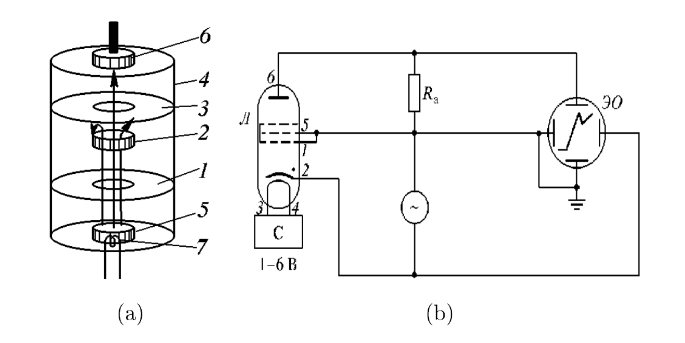
\includegraphics[width = 0.5\textwidth]{img/setup.png}
                \caption{Схема экспериментальной установки}
                \label{setup1}
            \end{center}
        \end{figure}

        Лампа-тиратрон ТГ3-01/1.3Б, заполненная инертным газом, расположена непосредственно на корпусе блока источника питания (БИП).
        Напряжение к электродам лампы подаётся от источников питания, находящихся в корпусе прибора.
        Регулировка напряжения и выбор режима работы установки производится при помощи ручек управления, выведенных на лицевую панель БИП.


        Зависимость вероятности рассеяния электрона от его энергии можно определить, зная ВАХ тиратрона:
        \begin{equation}
            \label{eq:w}
            w(U) = -\frac{1}{C}\ln \frac{I_a(U)}{I_0},
        \end{equation}
        где $I_0$ -- ток катода, а $C$ -- некоторая постоянная.

        По классическим представлениям, сечение рассеяния электрона на атоме должно падать монотонно с ростом $V$, как это показано на рисунке \ref{img:probability}а. По квантовым соображениям вероятность рассеяния электронов и соответствующая ВАХ должны иметь вид, показанный на рис. \ref{img:probability}б.

        \begin{figure}[h!]
            \begin{center}
                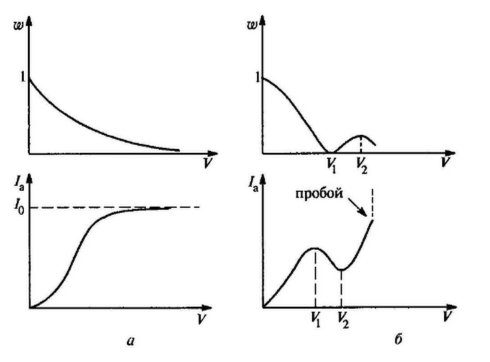
\includegraphics[width = 0.5\textwidth]{img/probability.png}
                \caption{Вероятность рассеяния электрона атомом инертного газа и ВАХ тиратрона при классическом (а) и квантовом (б) рассмотрении}
                \label{img:probability}
            \end{center}
        \end{figure}

    \section{Ход работы}

        \subsection{Динамический режим работы}

            Включим динамический режим и установим напряжение накала лампы равное $(3.07 \pm 0.01) \text{ В}$.

            Подкручивая ручкой фазу, сведём прямой и обратной ход характеристик.

            Измерим напряжение между сеткой и катодом, которое соответствует максимуму, минимуму харастеристик и пробою тиратрона. Ноль напряжения определяем при заземлении входа.

            Повторим измерения для напряжение накала лампы $(2.88 \pm 0.01) \text{ В}$.

            \begin{figure}[h!]
                    \centering
                    \subfloat[\centering $U_{\text{нак}} = (3.07 \pm 0.01) \text{ В}$.]{{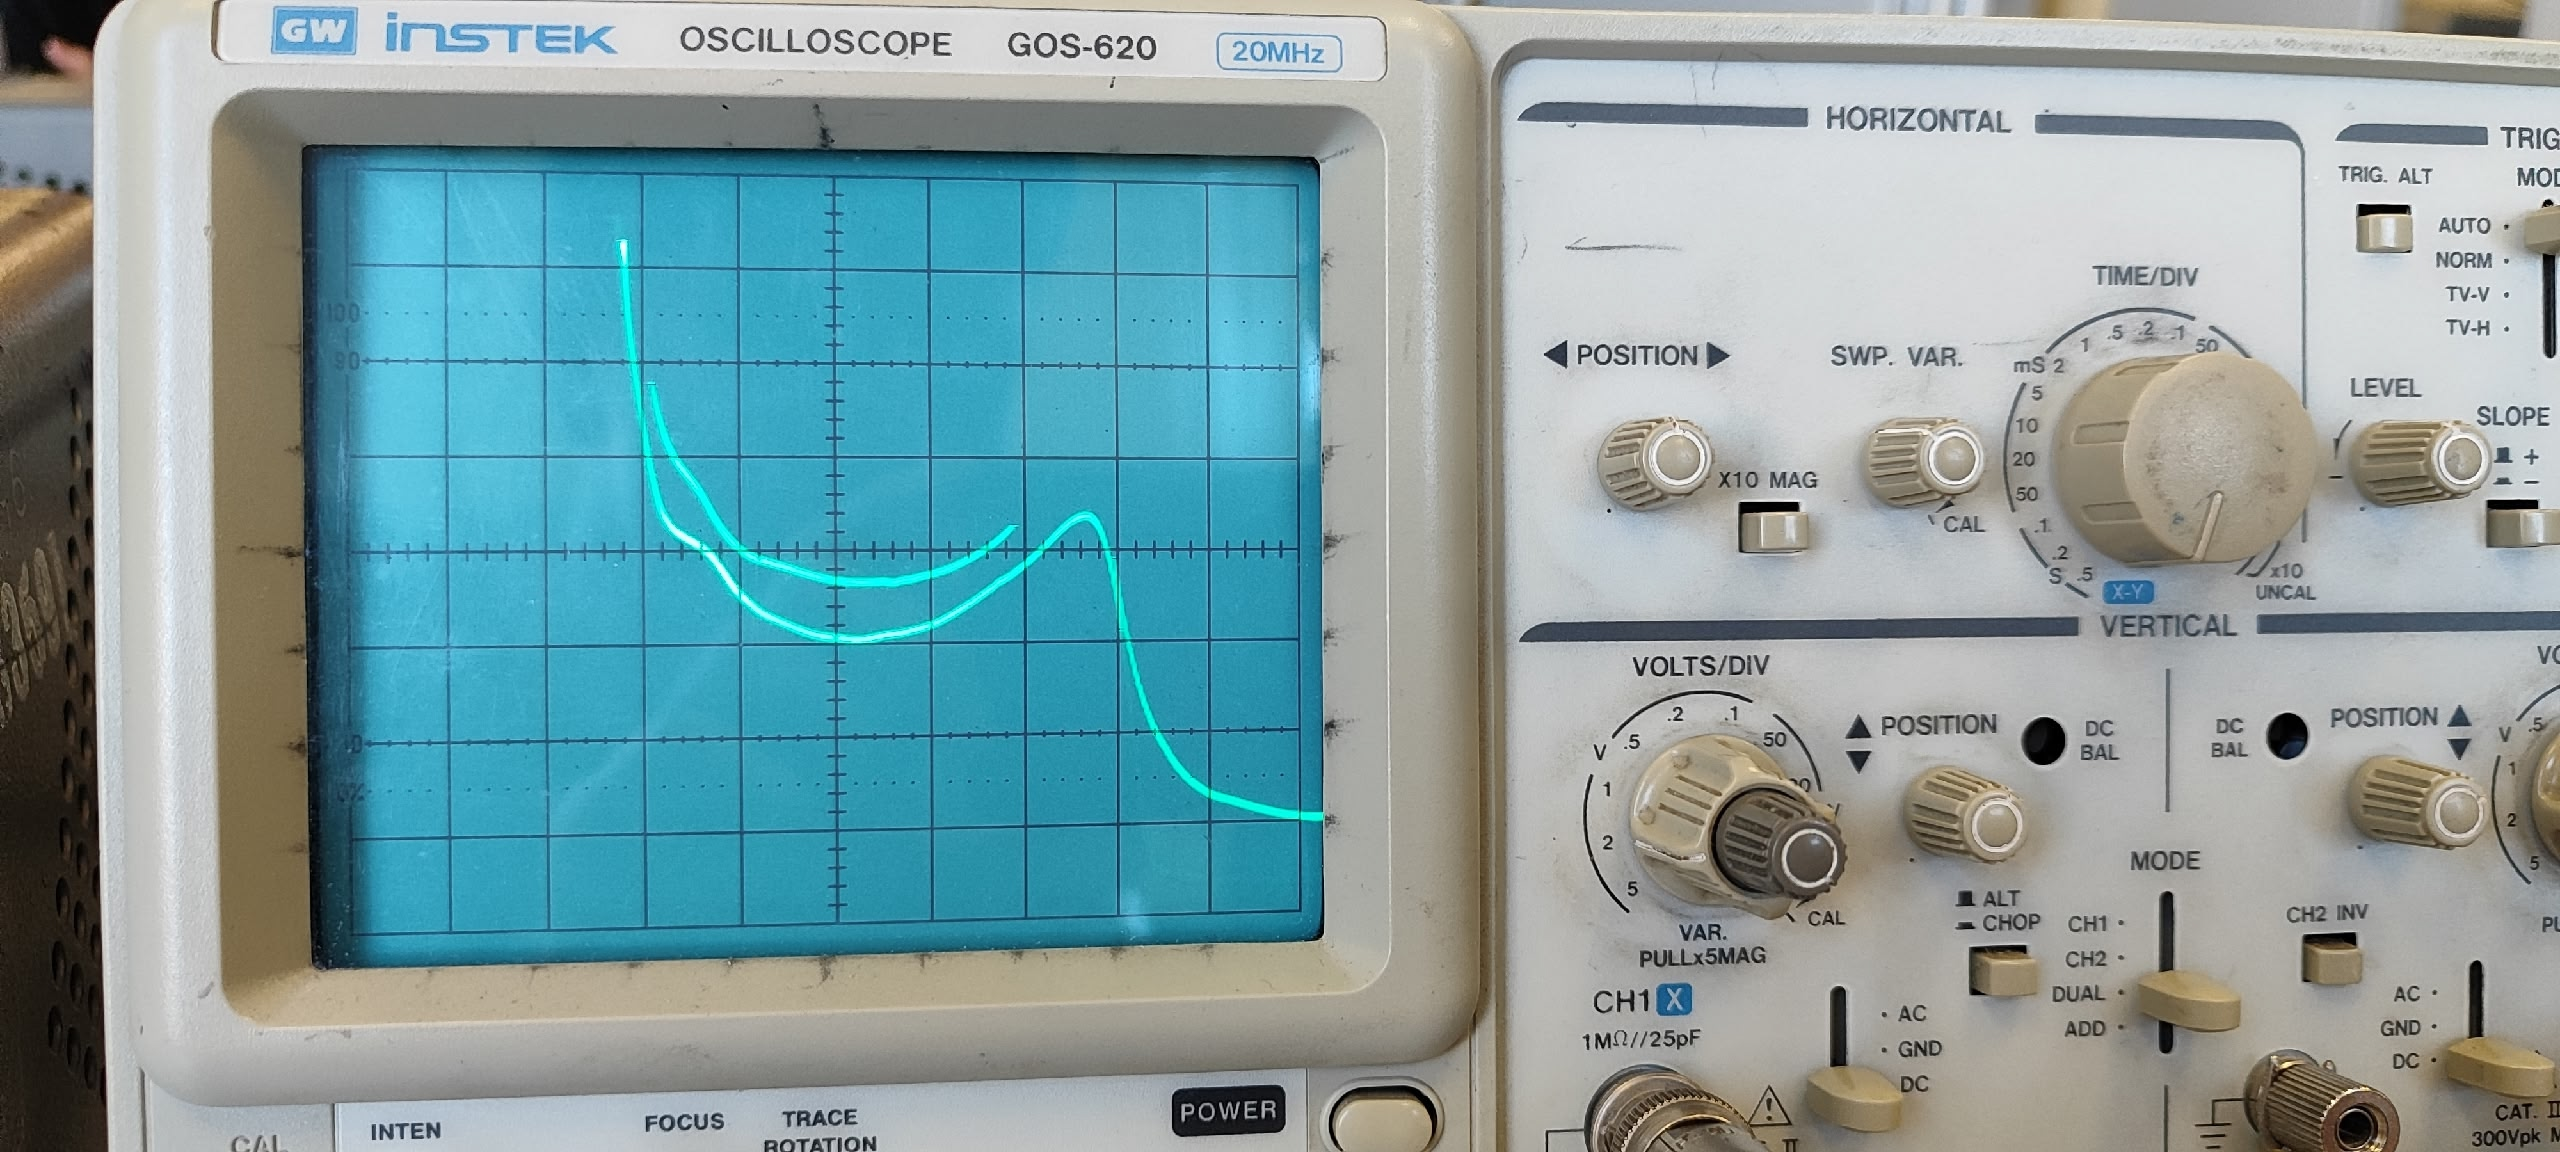
\includegraphics[width=0.45\linewidth]{img/dynamic_3.07.jpg}}}
                    \qquad
                    \subfloat[\centering $U_{\text{нак}} = (2.88 \pm 0.01) \text{ В}$.]{{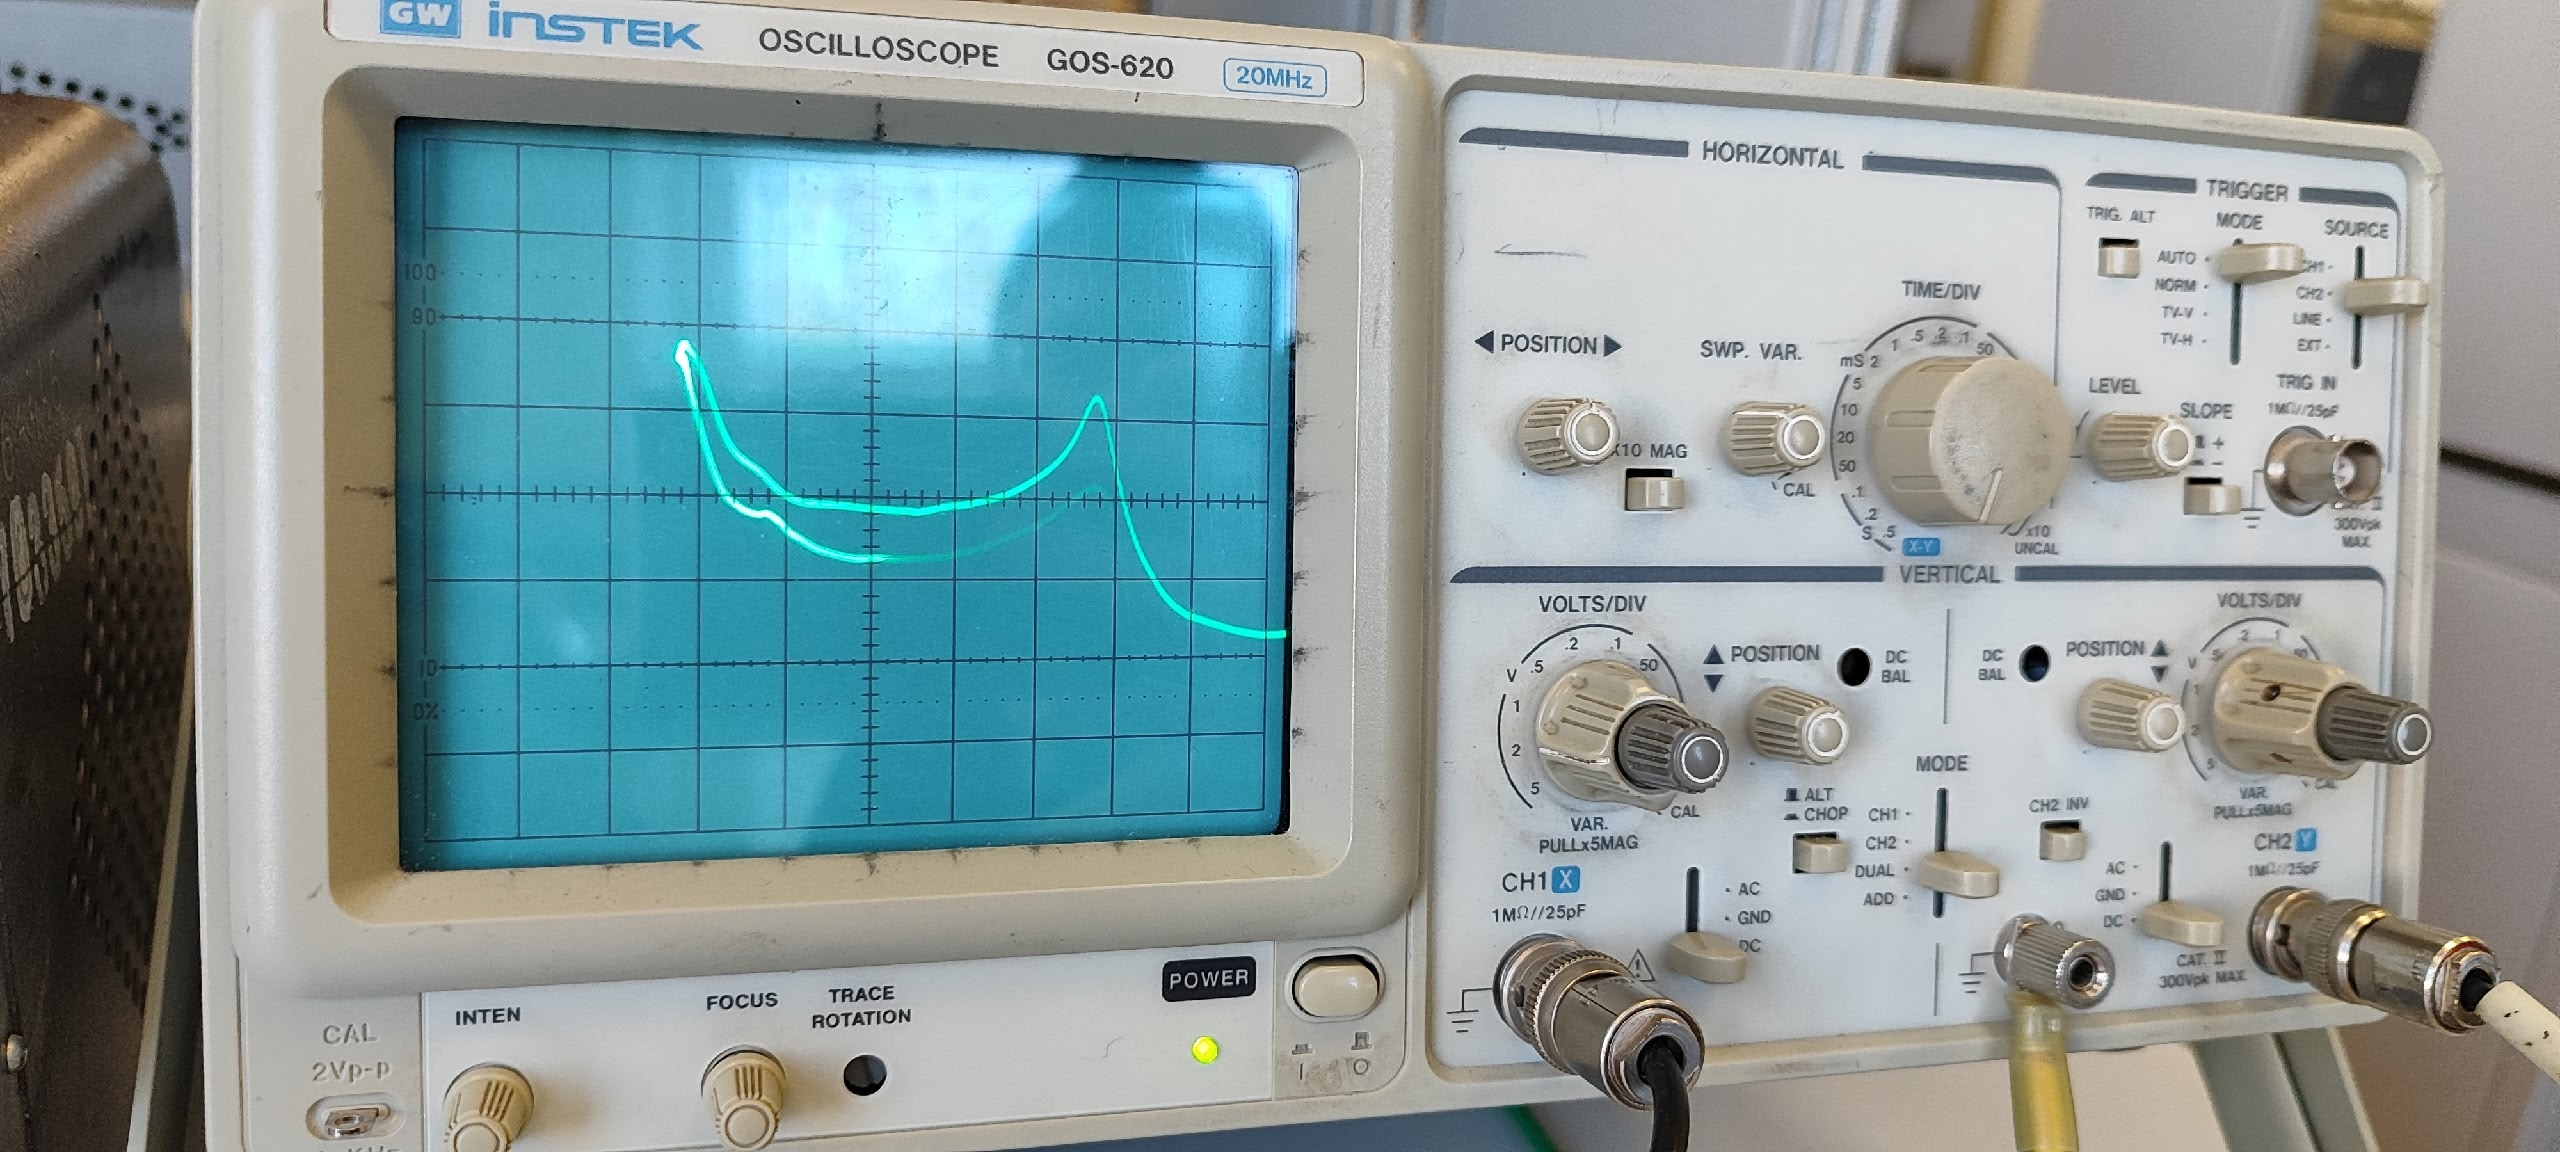
\includegraphics[width=0.45\linewidth]{img/dynamic_2.88.jpg}}}
                    \caption{ВАХ тиратрона}%
                    \label{fig:example}%
            \end{figure}

            \begin{table}[!ht]
                \centering
                \begin{tabular}{|c|c|c|c|}
                    \hline

                    $U_{накала}, В$ & $V_{max}, В$ & $V_{min}, В$ & $V_{пробоя}, В$\\ \hline
                    $3.07 \pm 0.01$ & $3.0 \pm 0.4$ & $8 \pm 1$ & $11.6 \pm 0.4$\\ \hline
                    $2.88 \pm 0.03$ & $2.4 \pm 0.4$ & $8 \pm 2$ & $11.6 \pm 0.4$\\ \hline

                \end{tabular}
                \caption{Результаты измерений в динамическом режиме}
               \label{}
            \end{table}

            По результатам измерений в динамическом режиме рассчитаем размер электронной оболочки атома инертного газа, заполняющего лампу по формуле $\eqref{eq:3}$, исключив $U_0$.

    \[ l = \frac{h\sqrt{5}}{\sqrt{32m(E_2-E_1)}}, ~\sigma_{l} = l \frac{\sigma_{E_2} + \sigma_{E_1}}{2(E_2 - E_1)}\]

            Оценим глубину потенциальной ямы по формуле $\eqref{eq:U_0}$.

            По результатам напряжения пробоя, оценим потенциал ионизации инертного газа. Наиболее близкое значение у ксенона -- $12.1 \text{ эВ}$

            \begin{table}[!ht]
                \centering
                \begin{tabular}{|c|c|c|c|}
                    \hline

                    $U_{нак}, В$ & $l, \textup{~\AA}$ & $U_0, эВ$ & $U_{проб}, эВ$\\ \hline
                    $3.070 \pm 0.010$ & $3.2 \pm 0.4$ & $-1 \pm 1$ & $11.6 \pm 0.4$\\ \hline
                    $2.88 \pm 0.03$ & $3.0 \pm 0.6$ & $-2 \pm 2$ & $11.6 \pm 0.4$\\ \hline

                \end{tabular}
                \caption{Результаты динамического способа}
                \label{tab:dynamic_res}
            \end{table}

        \subsection{Статический режим работы}

            Перейдем к измерению ВАХа в статическом режиме.

            Ток на аноде определяется по показанию вольтметра $(V_{\text{анод}})$, делённому на сопротивление $100 \text{ кОм}$, которое включено в цепь анода. $\sigma_{V_{\text{анод}}} = 0.01 \text{ мВ}$.

            Построим графики $V_{анод} = f(V_{катод})$.

            \begin{figure}[!ht]
                \centering
                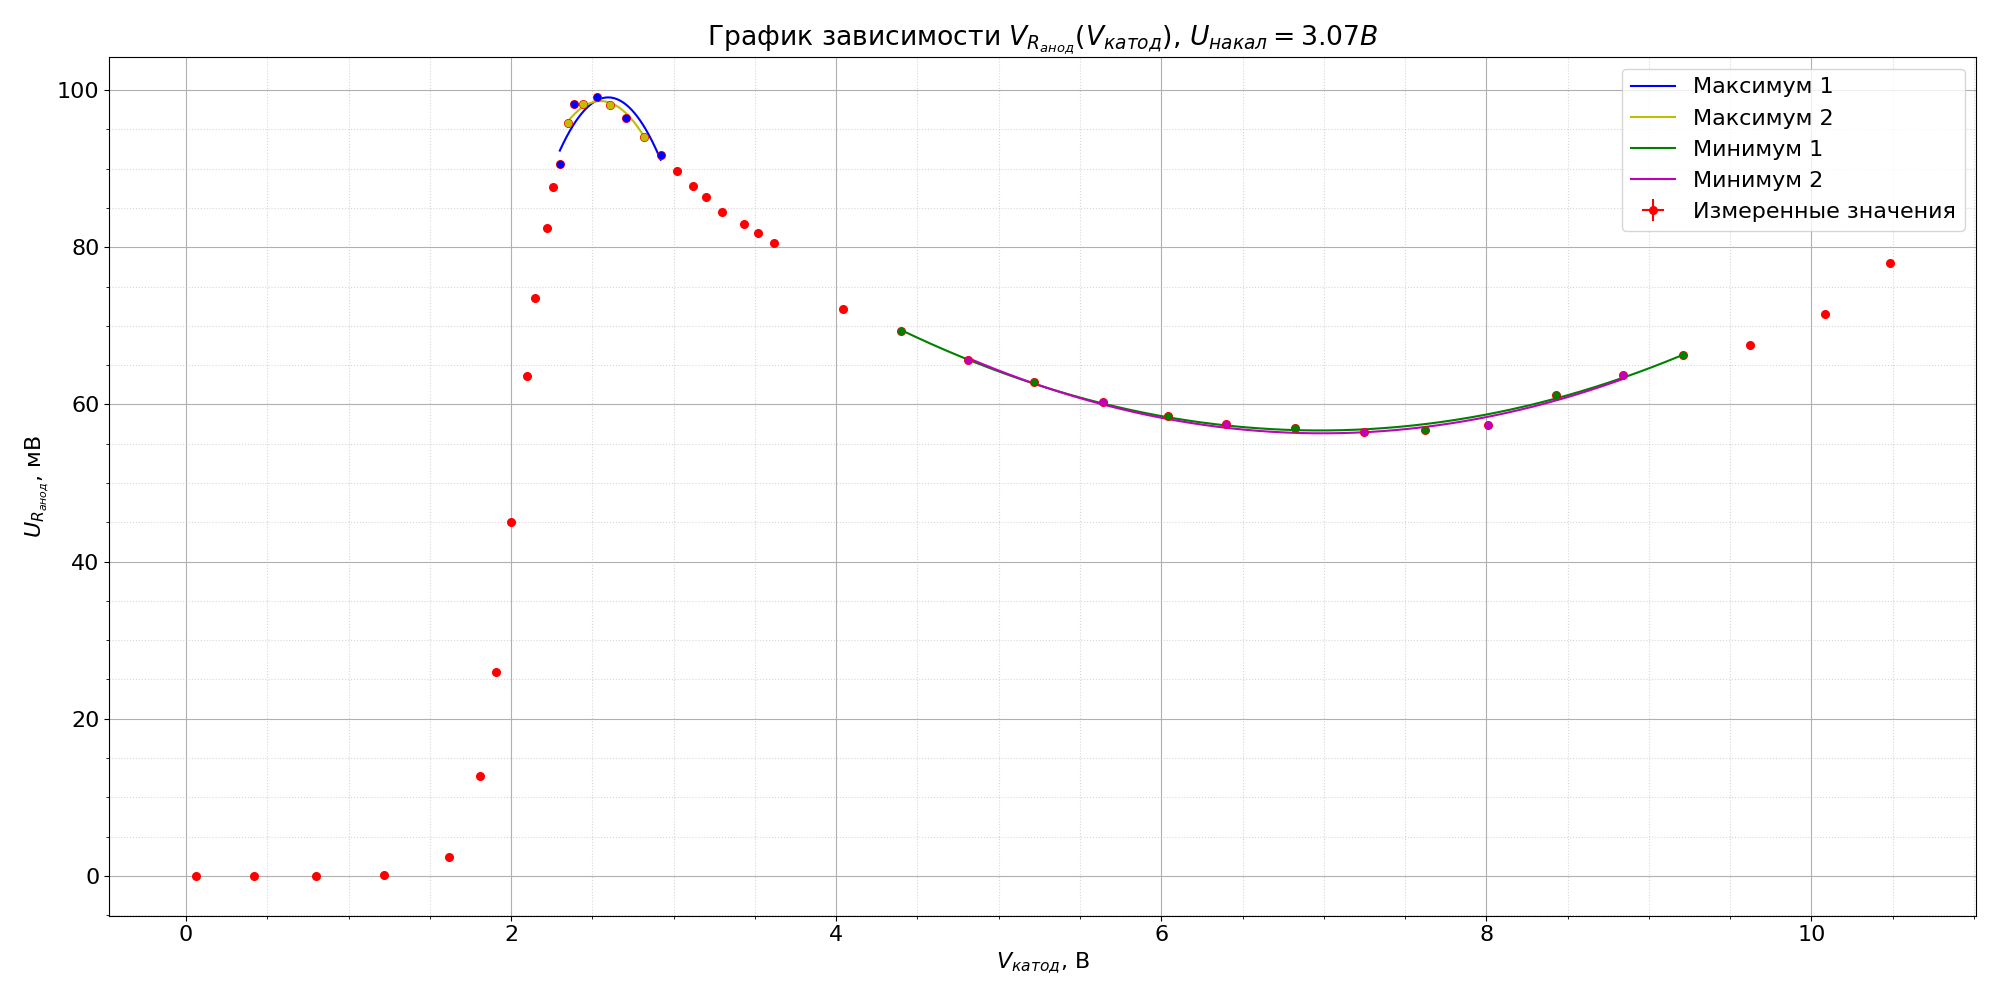
\includegraphics[width = 0.9\linewidth]{img/plot_static_3.07.png}
                \caption{Результаты статического режима для $U_{накала} = 3.07В$}
                \label{}
            \end{figure}

            \begin{figure}[!ht]
                \centering
                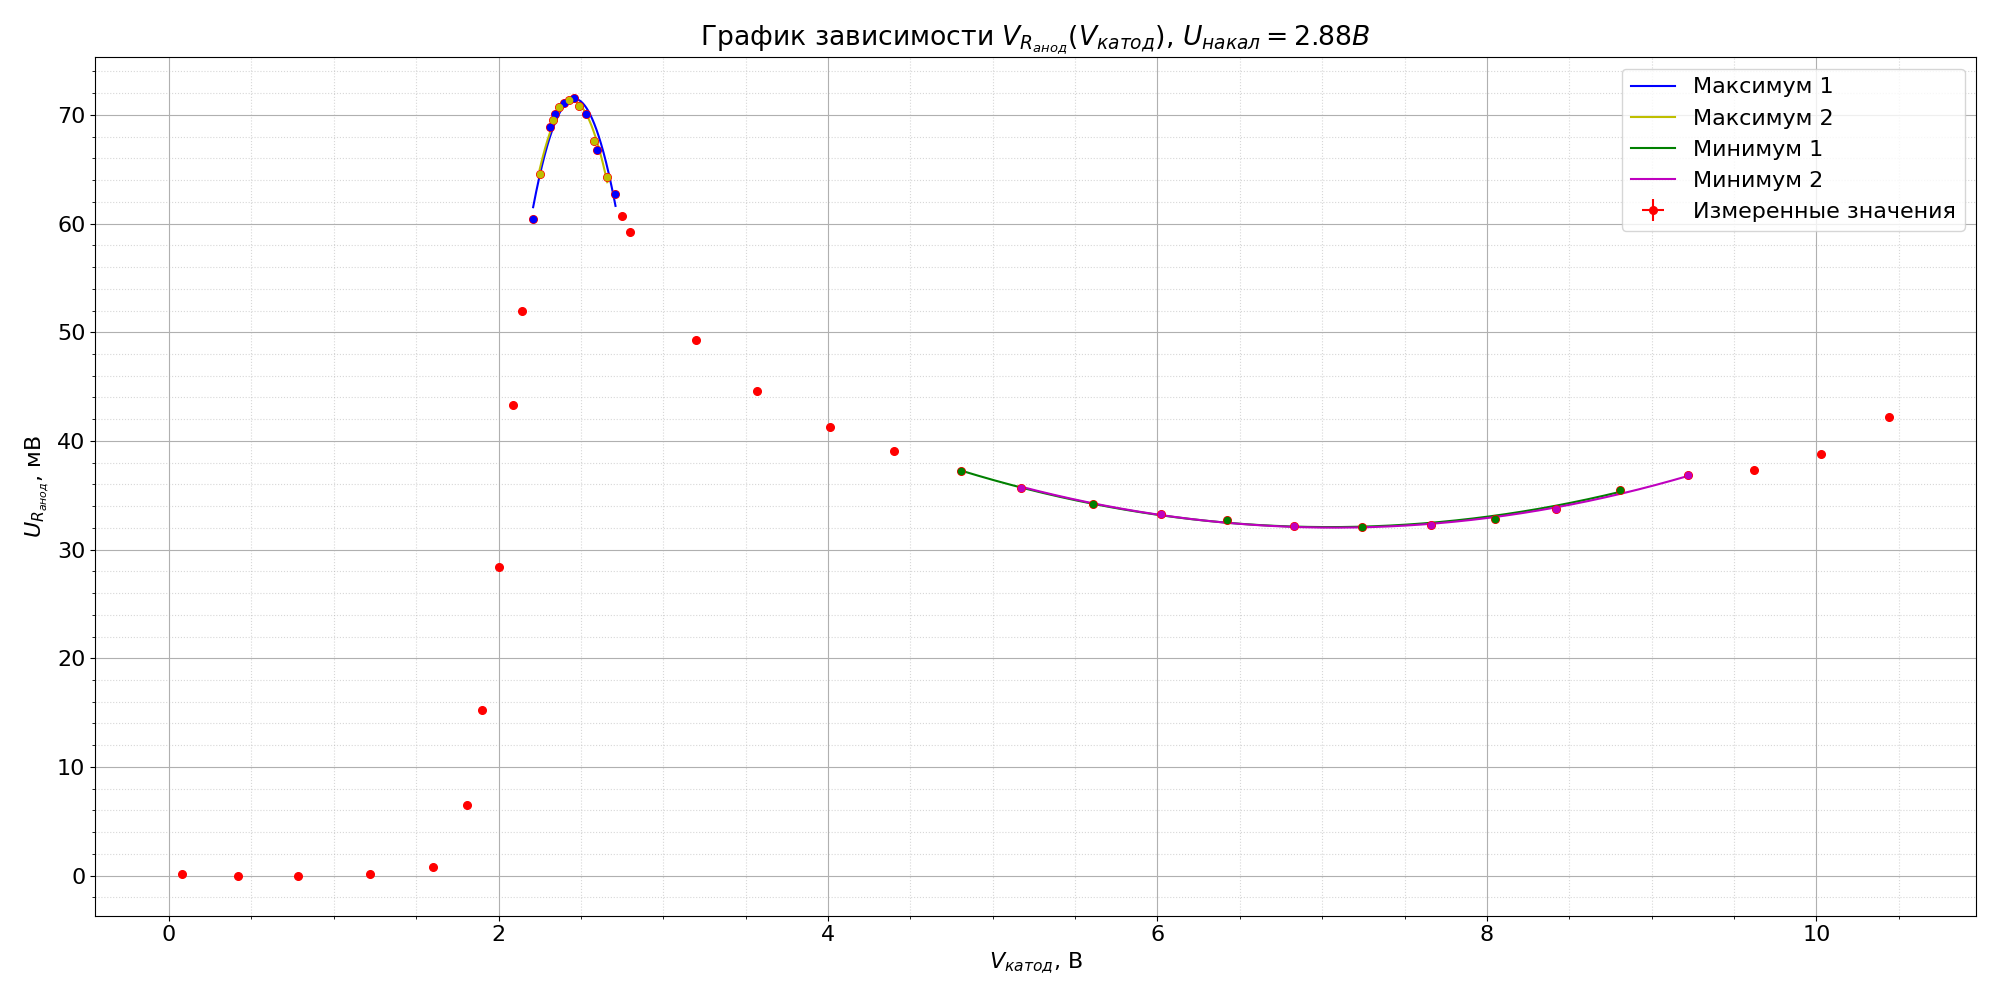
\includegraphics[width = 0.9\linewidth]{img/plot_static_2.88.png}
                \caption{Результаты статического режима для $U_{накала} = 2.88В$}
                \label{}
            \end{figure}

            Аппроксимируем пики графиков двумя параболами -- по чётным и нечётным точкам пика. За результат определения $V_{катод}$ возьмём среднее для двух парабол. Погрешность -- разность между двумя результатами.

            \begin{table}[!ht]
                \centering
                \begin{tabular}{|c|c|c|}
                    \hline

                    $U_{накала}, В$ & $V_{max}, В$ & $V_{min}, В$\\ \hline
                    $3.07 \pm 0.01$ & $2.57 \pm 0.05$ & $6.982 \pm 0.012$\\ \hline
                    $2.88 \pm 0.03$ & $2.45 \pm 0.01$ & $7.06 \pm 0.04$\\ \hline

                \end{tabular}
                \caption{Результаты измерений в статическом режиме}
                \label{}
            \end{table}

            \begin{table}[!ht]
                \centering
                \begin{tabular}{|c|c|c|}
                    \hline

                    $U_{накала}, В$ & $l, \textup{~\AA}$ & $U_0, эВ$\\ \hline
                    $3.07 \pm 0.01$ & $3.27 \pm 0.02$ & $0.95 \pm 0.09$\\ \hline
                    $2.88 \pm 0.03$ & $3.20 \pm 0.01$ & $1.23 \pm 0.04$\\ \hline

                \end{tabular}
                \caption{Результаты статического режима}
                \label{}
            \end{table}

            Оценим при каких напряжениях должны появляться максимумы в коэффециенте прохождения электронов для $n = 2, 3$
            \[ k_2 l = \sqrt{\frac{2m (E_n + U_0)}{\hbar^2}} l = n \pi ~\Rightarrow~ E_n = - U_0 + \frac{h^2 n^2}{8m l^2}\]

            Для оценки возьмём, как $U_0 = (-1.1 \pm 0.2) \text{ эВ}$ и $l = (3.23 \pm 0.04)$ \AA -- средние значения.
            \[ E_2 = (13.3 \pm 0.4) \text{ эВ}, ~E_3 = (31.4 \pm 0.8) \text{ эВ} \]

            Следующие максимумы выше потенциала ионизации, поэтому мы не можем их наблюдать.

            Найдём зависимость вероятности рассеяния электронов от энергии c точностью до константы C по формуле (\ref{eq:w}):

            \begin{figure}[h!]
                \centering
                \subfloat[\centering $U_{\text{накала}} = 3.07 \text{ В}$.]{{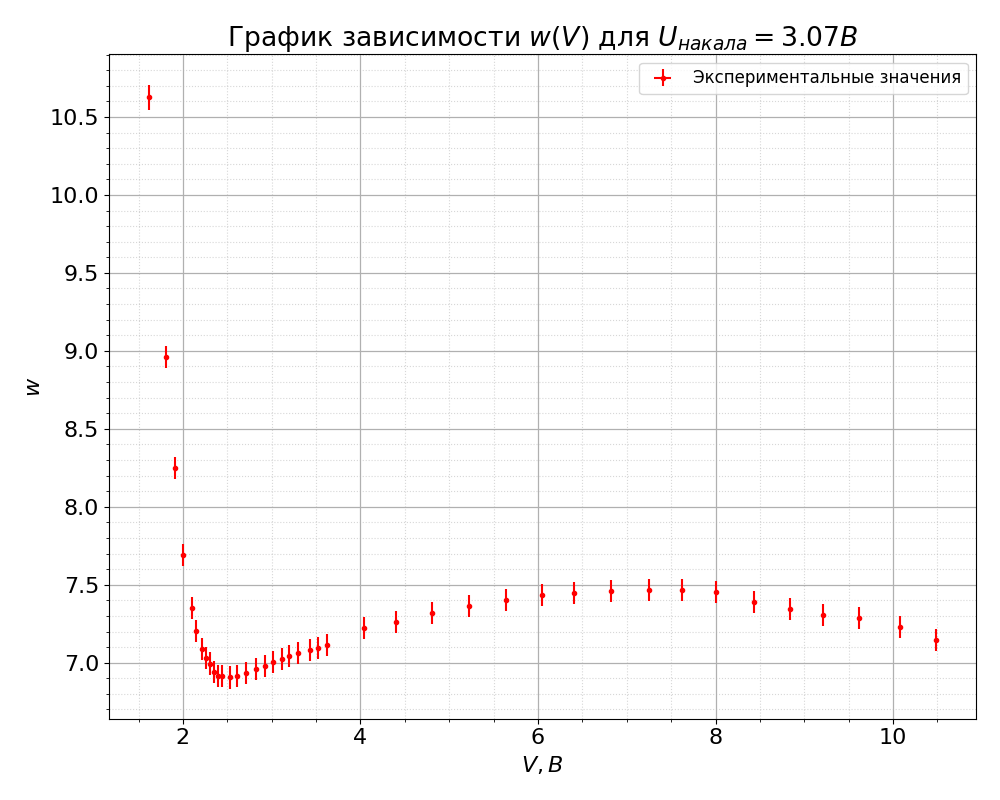
\includegraphics[width=0.45\linewidth]{img/plot_probability_3.07.png}}}%
                \qquad
                \subfloat[\centering $U_{\text{накала}} = 2.88 \text{ В}$.]{{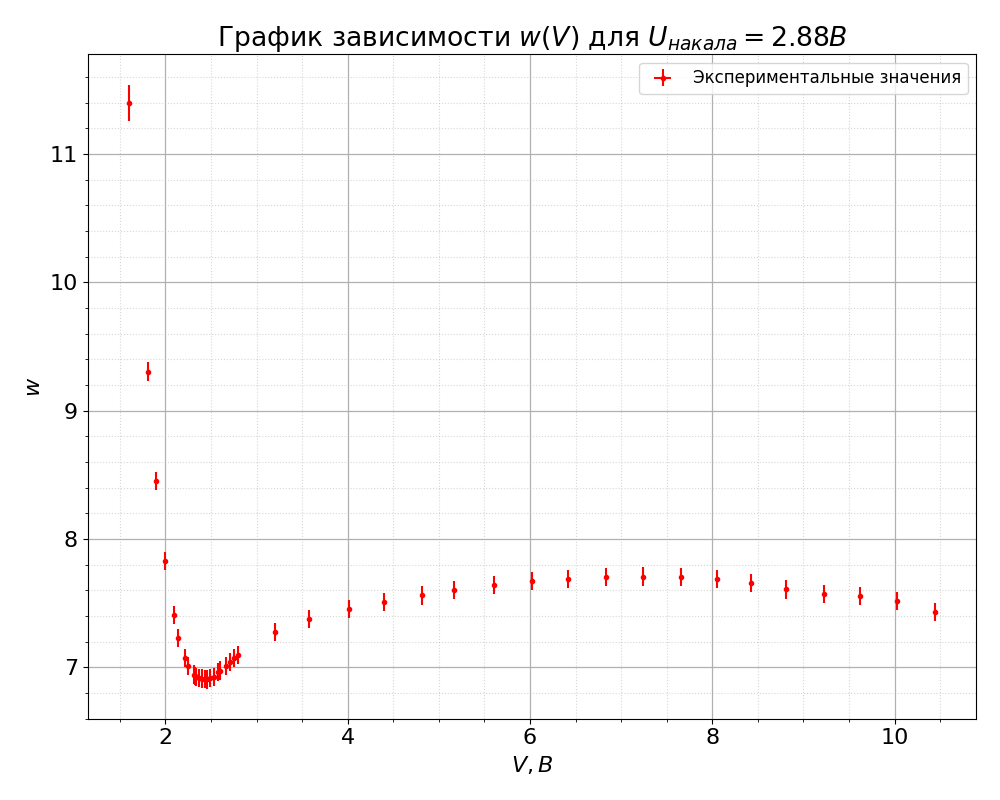
\includegraphics[width=0.45\linewidth]{img/plot_probability_2.88.png}}}%
                \caption{Зависимость вероятности рассеяния электрона от его энергии}%
            \end{figure}

    \section{Заключение}
        В ходе работы был изучен ВАХ тиратрона в динамическом и статическом режимах при различных напряжениях накала.

        С помощью измерений ВАХа тиратрона удалось установить, какой инертный газ использовался в работе: по напряжению пробоя была получена энергия ионизация газа, которая оказалась примерно равна энергии ионизации ксенона - $12.1 \text{ эВ}$.

        Также удалось оценить размер электронной оболочки разными метода, в среднем полученный результат $l = (3.23 \pm 0.04)$ \AA, что приблизительно соответствует значению для ксенона $l = 2.80$ \AA.
        А также глубину потенциальной ямы $U_0 = (- 1.1 \pm 0.2) \text{ эВ}$. Полученное значение показывает, что для подсчёта истинного значения требуется применения другой модели.

        \begin{table}[!ht]
            \centering
            \begin{tabular}{|c|c|c|c|}
                \hline

                $U_{нак}, В$ & $l, \textup{~\AA}$ & $U_0, эВ$ & $U_{проб}, эВ$\\ \hline
                $3.070 \pm 0.010$ & $3.2 \pm 0.4$ & $-1 \pm 1$ & $11.6 \pm 0.4$\\ \hline
                $2.88 \pm 0.03$ & $3.0 \pm 0.6$ & $-2 \pm 2$ & $11.6 \pm 0.4$\\ \hline

            \end{tabular}
            \caption{Результаты динамического способа}
            \label{tab:dynamic_res}
        \end{table}

        \begin{table}[!ht]
            \centering
            \begin{tabular}{|c|c|c|}
                \hline

                $U_{накала}, В$ & $l, \textup{~\AA}$ & $U_0, эВ$\\ \hline
                $3.07 \pm 0.01$ & $3.27 \pm 0.02$ & $0.95 \pm 0.09$\\ \hline
                $2.88 \pm 0.03$ & $3.20 \pm 0.01$ & $1.23 \pm 0.04$\\ \hline

            \end{tabular}
            \caption{Результаты статического режима}
            \label{}
        \end{table}

        Определена зависимость вероятности рассеяния электрона от его энергии для разных напряжений накала.

    \section{Приложение}

\begin{table}[!ht]
    \centering
    \begin{tabular}{|c|c|}
        \hline

        $V_{катод}, В$ & $V_{анод}, мВ$\\ \hline
        $0.06$ & $0.0$\\ \hline
        $0.42$ & $0.0$\\ \hline
        $0.80$ & $0.0$\\ \hline
        $1.22$ & $0.1$\\ \hline
        $1.62$ & $2.4$\\ \hline
        $1.81$ & $12.7$\\ \hline
        $1.91$ & $25.9$\\ \hline
        $2.00$ & $45.1$\\ \hline
        $2.10$ & $63.6$\\ \hline
        $2.15$ & $73.5$\\ \hline
        $2.22$ & $82.5$\\ \hline
        $2.26$ & $87.7$\\ \hline
        $2.30$ & $90.6$\\ \hline
        $2.35$ & $95.8$\\ \hline
        $2.39$ & $98.2$\\ \hline
        $2.44$ & $98.3$\\ \hline
        $2.53$ & $99.1$\\ \hline
        $2.61$ & $98.1$\\ \hline
        $2.71$ & $96.4$\\ \hline
        $2.82$ & $94.1$\\ \hline
        $2.92$ & $91.8$\\ \hline
        $3.02$ & $89.7$\\ \hline
        $3.12$ & $87.8$\\ \hline
        $3.20$ & $86.4$\\ \hline
        $3.30$ & $84.5$\\ \hline
        $3.43$ & $83.0$\\ \hline
        $3.52$ & $81.8$\\ \hline
        $3.62$ & $80.5$\\ \hline
        $4.04$ & $72.1$\\ \hline
        $4.40$ & $69.3$\\ \hline
        $4.81$ & $65.6$\\ \hline
        $5.22$ & $62.8$\\ \hline
        $5.64$ & $60.3$\\ \hline
        $6.04$ & $58.5$\\ \hline
        $6.40$ & $57.5$\\ \hline
        $6.82$ & $57.0$\\ \hline
        $7.25$ & $56.5$\\ \hline
        $7.62$ & $56.7$\\ \hline
        $8.01$ & $57.4$\\ \hline
        $8.43$ & $61.2$\\ \hline
        $8.84$ & $63.8$\\ \hline
        $9.21$ & $66.3$\\ \hline
        $9.62$ & $67.6$\\ \hline
        $10.08$ & $71.5$\\ \hline
        $10.48$ & $78.0$\\ \hline

    \end{tabular}
    \quad
    \begin{tabular}{|c|c|}
        \hline

        $V_{катод}, В$ & $V_{анод}, мВ$\\ \hline
        $0.08$ & $0.1$\\ \hline
        $0.42$ & $0.0$\\ \hline
        $0.78$ & $0.0$\\ \hline
        $1.22$ & $0.1$\\ \hline
        $1.60$ & $0.8$\\ \hline
        $1.81$ & $6.5$\\ \hline
        $1.90$ & $15.2$\\ \hline
        $2.00$ & $28.4$\\ \hline
        $2.09$ & $43.3$\\ \hline
        $2.14$ & $52.0$\\ \hline
        $2.21$ & $60.4$\\ \hline
        $2.25$ & $64.6$\\ \hline
        $2.31$ & $68.9$\\ \hline
        $2.33$ & $69.5$\\ \hline
        $2.34$ & $70.1$\\ \hline
        $2.37$ & $70.7$\\ \hline
        $2.40$ & $71.1$\\ \hline
        $2.43$ & $71.4$\\ \hline
        $2.46$ & $71.6$\\ \hline
        $2.49$ & $70.8$\\ \hline
        $2.53$ & $70.1$\\ \hline
        $2.58$ & $67.6$\\ \hline
        $2.60$ & $66.8$\\ \hline
        $2.66$ & $64.3$\\ \hline
        $2.71$ & $62.7$\\ \hline
        $2.75$ & $60.7$\\ \hline
        $2.80$ & $59.2$\\ \hline
        $3.20$ & $49.3$\\ \hline
        $3.57$ & $44.6$\\ \hline
        $4.01$ & $41.3$\\ \hline
        $4.40$ & $39.1$\\ \hline
        $4.81$ & $37.2$\\ \hline
        $5.17$ & $35.7$\\ \hline
        $5.61$ & $34.2$\\ \hline
        $6.02$ & $33.3$\\ \hline
        $6.42$ & $32.7$\\ \hline
        $6.83$ & $32.2$\\ \hline
        $7.24$ & $32.1$\\ \hline
        $7.66$ & $32.3$\\ \hline
        $8.05$ & $32.8$\\ \hline
        $8.42$ & $33.7$\\ \hline
        $8.81$ & $35.5$\\ \hline
        $9.22$ & $36.9$\\ \hline
        $9.62$ & $37.3$\\ \hline
        $10.03$ & $38.8$\\ \hline
        $10.44$ & $42.2$\\ \hline

    \end{tabular}
    \caption{Результаты измерений для статического метода для $U_{накала} = 3.07 В$ и $U_{накала} = 2.88 В$}
    \label{}
\end{table}

\end{document}
